\section{Programming with the IBM ExaBounds API}
\label{sec:300:notebook}

IBM ExaBounds can be used with custom notebooks by programming in Mathematica while using the IBM ExaBounds API. This section describes how to the use API.

\subsection{Starting point}

As the starting point, one should always load the \textsc{ExaBoundsLite.nb} notebook and execute it contents. This will make sure all the packages are loaded and the data structures are initialized.

\subsection{Loading algorithms}

Algorithms can be loaded automatically without using the GUI. First, create a list of IBM Platform-Independent Software Analysis profile files (full path and filename) to load:
\begin{mma}
	\In |dir| = \mathtt{"}/home/user/\mathtt{"}; \\
  \In |JSONfileList| = \{ \linebreak
    |dir| <> \mathtt{"}app1.out\mathtt{"}, \linebreak
    |dir| <> \mathtt{"}app2.out\mathtt{"}, \linebreak
    |dir| <> \mathtt{"}app3.out\mathtt{"} \linebreak
  \}; \\
\end{mma}

The profile files in the list can now be loaded using \textsc{AddAlgorithm}:
\begin{mma}
  \In |algorithmIdentifiers| = \linebreak |AddAlgorithm|[|ExaBoundsAlgInfo|, \#]~\& /@ |JSONfileList|; \\
\end{mma}

The call to \textsc{AddAlgorithm[]} for each file returns a list of \textsc{algorithmIdentifiers}, each corresponding to the first data profile and first thread in the profile files (in the same order as the files in the file list). Each of the identifiers consists of four elements identifying the application, scaling parameter, data profile, and thread. Essentially, this is in an index into the drop-down boxes in Figure~\ref{fig:200:applicationpicker}. Note that the GUI elements in the \textsc{ExaBoundsLite.nb} notebook (e.g., Figure~\ref{fig:200:loadjson}) are also updated to reflect loading of the files.

IBM Exascale Extrapolator output files can be loaded as well automatically. One can use the \textsc{Get[]} to load the file subsequently followed by a call to \textsc{AppendAlgorithmAnalysis[]} to load the data into the IBM ExaBounds data structures:
\begin{mma}
  \In |Get|[\mathtt{"}/home/user/extrax-file.m\mathtt{"}]; \\
  \In |AppendAlgorithmAnalysis|[|ExaBoundsAlgInfo|, |predictedAlgorithm|]; \\
\end{mma}
Here, \textsc{ExaBoundsAlgInfo} is the name of the IBM ExaBounds data structure and \textsc{predictedAlgorithm} is the default name of the symbol defined in the IBM Exascale Extrapolator output file which contains the extrapolated application profiles.

For the network performance models, the user is required to set the communication pattern of the application. The pattern needs to be defined per process profile (if the profile is extracted from a IBM Platform-Independent Software Analysis) or per class (cluster) profile (if the profile is extracted from an extrapolated IBM Exascale Extrapolator file), even though the pattern is the same pattern for all processes or classes (clusters) of processes. If the communication pattern is not known a-priori, the user should manually examine the communication matrix that shows how much data the processes exchange among each other during the execution of the program. Currently IBM ExaBounds supports three types of HPC patterns: \textit{uniform} (uniform all-to-all), \textit{shift} (with shift value \textit{value}) and \textit{nne2D} (2-dimension nearest-neighbor with an application domain size of D1$\cdot$D2). The user can set the communication pattern as follows:

\begin{mma}
	\In |swProfile| = |ExaBoundsAlgInfo[algName][scalingConfiguration]| \linebreak |[[dataProfile]][{processId, 0}]|; \\
	\In |swProfile| = |SetKeyValue[swProfile|, \mathtt{"}|CommunicationPattern|\mathtt{"}, \linebreak
	<\mathtt{\mid"}|type|\mathtt{"} \rightarrow  \mathtt{"}|nne2D|\mathtt{"},  \mathtt{"}D1\mathtt{"} \rightarrow |D1|,  \mathtt{"}D2 \mathtt{"} \rightarrow |D2| \mathtt{\mid}>]; \\
	\In |swProfile| = |SetKeyValue[swProfile|, \mathtt{"}|CommunicationPattern|\mathtt{"}, \linebreak
	<\mathtt{\mid"}|type|\mathtt{"} \rightarrow  \mathtt{"}|shift|\mathtt{"},  \mathtt{"}value\mathtt{"} \rightarrow |value| \mathtt{\mid}>]; \\
	\In |swProfile| = |SetKeyValue[swProfile|, \mathtt{"}|CommunicationPattern|\mathtt{"}, \linebreak
	<\mathtt{\mid"}|type|\mathtt{"} \rightarrow  \mathtt{"}|uniform|\mathtt{"} \mathtt{\mid}>]; \\
\end{mma}

\subsection{Loading architectures}

Architectures can be automatically loaded using three functions that each take a path to the respective processor architecture, memory, or network JSON file:
\begin{mma}
\In |LoadArchJSON|[|jsonFile|]; \\
\In |LoadMemJSON|[|jsonFile|]; \\
\In |LoadNetworkJSON|[|jsonFile|]; \\
\end{mma}

In order to use \textsc{LoadMemJSON[]} the package \textsc{PreDefinedMemorySpec`} has to be manually loaded.

\subsection{Selecting and modifying architectures}

An architecture can be selected from the predefined configurations by overwriting the \textsc{ExaBoundsState} variable as:
\begin{mma}
  \In |architectureString| = \mathtt{"}T4240\mathtt{"}; \\
  \In |ExaBoundsState| = |ExaBoundsMergeState|[|ExaBoundsState|, \linebreak |predefinedconfig|[|architectureString|, \mathtt{"}\mathtt{"}]]; \\
\end{mma}

The \textsc{predefinedconfig[]} retrieves the architectural properties of the specified architecture. However, it may only specify a subset of the required properties. As a result, it needs to be merged (\textsc{ExaBoundsMergeState[]}) with the existing properties in \textsc{ExaBoundsState} to make sure that all properties are available and have some default value. The second argument of \textsc{predefinedconfig[]} is deprecated.

The \textsc{architectureString} identifies the architecture from the list of predefined architectures. The predefined architectures can be found in the \textsc{PreDefinedMachineConfigs.m} package or by inspection:
\begin{mma}
  \In |predefinedConfigID2Name| \\
  \Out \{\mathtt{"}IBM8236-E8C\mathtt{"} \rightarrow \mathtt{"}IBM 8236-E8C (four-socket Power7)\mathtt{"}, \linebreak\mathtt{"}PowerLinux-7R2\mathtt{"} \rightarrow \mathtt{"}PowerLinux 7R2 (two-socket POWER7+)\mathtt{"}, ... \\
\end{mma}

It is possible to change architectural parameters using \textsc{SetKeyValue[]};
\begin{mma}
  \In |ExaBoundsState| = |SetKeyValue|[|ExaBoundsSate|,\mathtt{"}n1\mathtt{"},16]; \\
\end{mma}
This example sets the core count to 16. To inspect a parameter:
\begin{mma}
  \In |GetKeyValue|[|ExaBoundsSate|,\mathtt{"}n1\mathtt{"}] \\
  \Out 16 \\
\end{mma}
Other examples for changing the architecture are provided below specifically for the network parameters. \\

To change the name of the network topology to full-mesh:
\begin{mma}
	\In |ExaBoundsState| = |SetKeyValue|[|ExaBoundsSate|, \linebreak \mathtt{"}|networkConfiguration|\mathtt{"}, \mathtt{"}|full\mathtt{-}mesh|\mathtt{"}]; \\
\end{mma}
To change the description of the network topology:
\begin{mma}
	\In |ExaBoundsState| = |SetKeyValue|[|ExaBoundsSate|, \linebreak \mathtt{"}|topologyDescription|\mathtt{"}, \mathtt{"}|full\mathtt{-}mesh|\mathtt{"}, 
	<\mathtt{\mid"}|a|\mathtt{"} \rightarrow  |a|,  \mathtt{"}p\mathtt{"} \rightarrow |p| \mathtt{\mid}>]; \\
\end{mma}
To change the end node MPI stack latency:
\begin{mma}
	\In |ExaBoundsState| = |SetKeyValue|[|ExaBoundsSate|, \linebreak \mathtt{"}|nodeStackLatency|\mathtt{"}, |0.000001|]; \\
\end{mma}
To change the node-to-switch link bandwidth:
\begin{mma}
	\In |ExaBoundsState| = |SetKeyValue|[|ExaBoundsSate|, \linebreak \mathtt{"}|nodeSwitchBandwidth|\mathtt{"}, |5*1024*1024*1024|]; \\
\end{mma}
To change the mapping of the MPI processes for the \textit{uniform} or \textit{shift} pattern:
\begin{mma}
	\In |ExaBoundsState| = |SetKeyValue|[|ExaBoundsSate|, \linebreak \mathtt{"}|mappingDescription|\mathtt{"}, <\mathtt{\mid"}|type|\mathtt{"} \rightarrow  \mathtt{"}|linear|\mathtt{"} \mathtt{\mid}>]; \\
\end{mma}
To change the mapping of the MPI processes for the 2-dimension nearest-neighbor \textit{nne2D} pattern for the full-mesh or fat-tree-2L network topology (more information about the mapping is provided in Appendix~\ref{app:architecture-parameters}):
\begin{mma}
	\In |ExaBoundsState| = |SetKeyValue|[|ExaBoundsSate|, \mathtt{"}|mappingDescription|\mathtt{"}, \linebreak <\mathtt{\mid"}|type|\mathtt{"} \rightarrow  \mathtt{"}|linear|\mathtt{"},  \mathtt{"}d11\mathtt{"} \rightarrow |d11|, \mathtt{"}d12\mathtt{"} \rightarrow |d12| \mathtt{\mid}>]; \\
\end{mma}

\subsection{Performing a single-thread single-node experiment}

\begin{minipage}[t]{0.05\textwidth}
~\\
\Huge !
\end{minipage}
\begin{minipage}[t]{0.94\textwidth}
Before starting an experiment it is key to realize that the processor architecture parameters are for a specific vector width while the loaded algorithm profiles are for an unspecified vector width. Therefor, one should \emph{always} first convert an application profile to match the architected vector width of the target processor architecture. There are no exceptions, this also needs to be done for processor architectures without vector units: in that case, the profiles are converted to have only scalar instructions.
\end{minipage}
~\linebreak

First, we define a wrapper function that converts our profiles for the correct vector width and then calls an appropriate function in IBM ExaBounds to predict the behavior of the application. In this example, we are interested in the compute execution time in seconds:
\begin{mma}
  \In |ExecutionTimeWrapper|[|archProperties|\_, |algProperties|\_] := \linebreak
  |Block|[\{|convertedAlgProperties|\}, \linebreak
  \quad|convertedAlgProperties| = \linebreak
  \quad\quad|GetAlgorithmVectorProperties|[|archProperties|, \linebreak \quad\quad\quad |algProperties|]; \linebreak
  \quad|Return|[\linebreak\quad\quad|ExecutionSeconds|[|archProperties|, |convertedAlgProperties|]\linebreak\quad]; \linebreak
  ]; \\
\end{mma}

In this example, we first create a wrapper function called \textsc{ExecutionTimeWrapper[]} that takes as input a set of architectural and application properties. First, we convert the application properties to match the architecture using \textsc{GetAlgorithmVectorProperties[]} and store this in a temporary variable. Finally, we call \textsc{ExecutionSeconds[]} to predict the execution time and we return the results. A list of potential model calls is listed in Table~\ref{tbl:300:modelapi}.

Finally, we can call the wrapper function for every algorithm we loaded to get a list of execution times:
\begin{mma}
  \In |executionTimeList| =  |ExecutionTimeWrapper|[|ExaBoundsState|, \linebreak |GetAlgorithmKeyValueList|[|ExaBoundsAlgInfo|, \#]]~\& /@ \linebreak |algorithmIdentifiers| \\
  \Out \{6.43, 12.79, 8.63\} \\
\end{mma}

\begin{sidewaystable}
 \centering
 \small
 \caption{List of model API calls. All functions return values for a single thread.}
 \label{tbl:300:modelapi}
 \begin{threeparttable}
   \begin{tabular}{ll}
     \toprule
     \textbf{Function} & \textbf{Description} \\
     \midrule
     PeakFLOPSi[i\_, archProperties\_] & Peak performance in FLOPS at layer $i$\tnote{1} \\
     AchievedFLOPSi[i\_, archProperties\_, algProperties\_] & Achieved performance in FLOPS at layer $i$\tnote{2} \\
     d0Optimize[archProperties\_, algProperties\_] & Achieved CPI \\
     ExecutionCycles[archProperties\_, algProperties\_] & Total execution cycles \\
     ExecutionSeconds[archProperties\_, algProperties\_] & Total execution seconds \\
     FiMem[cacheLevel\_, archProperties\_, algProperties\_] & Fraction of total instruction to a certain cache level \\
     \midrule
     Poweri[i\_, archProperties\_, algProperties\_] & Power on layer $i$ \\
     PoweriMemory[i\_, archProperties\_, algProperties\_] & Memory power on layer $i$ \\
     AreaProcessor[archProperties\_, algProperties\_] & Processor area from McPAT \\
     \bottomrule
    \end{tabular}
    \begin{tablenotes}
      \item[1] See Table~\ref{tbl:300:levels} for helper functions to specify the right cache levels and architecture layers.
      \item[2] Currently only valid at the core layer.
    \end{tablenotes}
  \end{threeparttable}
\end{sidewaystable}

\begin{table}
 \centering
 \small
 \caption{List of helper functions to identify levels and layers.}
 \label{tbl:300:levels}
 \begin{tabular}{ll}
   \toprule
   \textbf{Function} & \textbf{Description} \\
   \midrule
   CoreLayer[] & Core layer \\
   DieLayer[] & Die layer \\
   SocketLayer[] & Socket layer \\
   CardLayer[] & Card layer \\
   RackUnitLayer[] & Rack unit layer \\
   RackLayer[] & Rack layer \\
   AisleLayer[] & Aisle layer \\
   SystemLayer[] & System layer \\
   \midrule
   MemoryL1Cache[] & Private L1 cache level \\
   MemoryL2Cache[] & Private L2 cache level \\
   MemoryL3Cache[] & Shared L3 cache level \\
   MemoryDRAM[] & DRAM level \\
   \bottomrule
  \end{tabular}
\end{table} 

\subsection{Performing a multi-core single-node experiment}

For a multi-core experiment we estimate the individual performance of a single thread using the single-core model~\cite{Jongerius2016}. To model congestion on the L3 cache and the memory bandwidth, we calculate the effective L3 cache size of each thread and evaluate the single-core model using the effective L3 cache size as the L3 size. Finally, we scale the results such that the total DRAM bandwidth of all threads on a processor does not exceed the maximum bandwidth.

\subsubsection{Using the single-core models}

We calculate the effective cache sizes by using \textsc{SolveCachePressure[]}. This function takes as argument the architecture properties as well as a mapping of algorithm profiles. The mapping can either be a list (for a fully custom mapping) or a single profile. In the latter case, it assumes that each core executes the same profile. As an example, consider the case where we wish to run two threads on a processor. This processor has 2 cores, each with a L1 cache of 32\,kB, an L2 cache of 256\,kB and a L3 cache of 4096\,kB:
\begin{mma}
 \In |profile1| = |GetAlgorithmKeyValueList|[|ExaBoundsAlgInfo|, \linebreak|algorithmIdentifiers|[[1]]]; \\
 \In |profile2| = |GetAlgorithmKeyValueList|[|ExaBoundsAlgInfo|, \linebreak|algorithmIdentifiers|[[2]]]; \\
 \In |mapping| = \{1 \rightarrow |profile1|, 2 \rightarrow |profile2|\}; \\
 \In |pressures| = |SolveCachePressure|[|ExaBoundsState|, |mapping|] \\
 \Out \{1 \rightarrow \{\mathtt{"}M0L1\mathtt{"} \rightarrow 32 * 1024, \mathtt{"}M0L2\mathtt{"} \rightarrow 256 * 1024, \mathtt{"}M1\mathtt{"} \rightarrow 1024 * 1024\}, 2 \rightarrow \{\mathtt{"}M0L1\mathtt{"} \rightarrow 32 * 1024, \mathtt{"}M0L2\mathtt{"} \rightarrow 256 * 1024,  \mathtt{"}M1\mathtt{"} \rightarrow 3072 * 1024\}\} \\
\end{mma}

The returned values are the effective caches sizes for each of the three layers of cache. Each thread has the full size of the private caches per core (\textsc{M0L1} and \textsc{M0L2}) available, while only part of the size of the shared L3 (\textsc{M1}). Now, we determine the performance of each thread. Note that this does not account for a thread finishing early and freeing resources for other threads to use. We can determine the execution time as:
\filbreak\begin{mma}
 \In |app| = 1; \\
 \In |ExaBoundsState| = |SetKeyValue|[|ExaBoundsState|, \mathtt{"}M1\mathtt{"}, \linebreak\mathtt{"}M1\mathtt{"}\!/.\!|pressures|[[|app|, 2]]]; \\
 \In |executionTimeApp1| =  \linebreak|ExecutionTimeWrapper|[|ExaBoundsState|, |profile1|] \\
 \Out 4.23 \\
 \In |app| = 2; \\
 \In |ExaBoundsState| = |SetKeyValue|[|ExaBoundsState|, \mathtt{"}M1\mathtt{"}, \linebreak\mathtt{"}M1\mathtt{"}\!/.\!|pressures|[[|app|, 2]]]; \\
 \In |executionTimeApp2| =  \linebreak|ExecutionTimeWrapper|[|ExaBoundsState|, |profile2|] \\
 \Out 8.23 \\
\end{mma}

\subsubsection{Using the multi-core models}

An easier method is to use the multi-core models available in IBM ExaBounds. These functions automatically calculate the cache pressures and return a list of values, one for each thread. We get the profiles, convert them for the right vector architecture and create a mapping similar as before:
\begin{mma}
 \In |profile1| = |GetAlgorithmVectorProperties|[|archProperties|, \linebreak |GetAlgorithmKeyValueList|[|ExaBoundsAlgInfo|, \linebreak|algorithmIdentifiers|[[1]]]]; \\
 \In |profile2| = |GetAlgorithmVectorProperties|[|archProperties|, \linebreak|GetAlgorithmKeyValueList|[|ExaBoundsAlgInfo|, \linebreak|algorithmIdentifiers|[[2]]]]; \\
 \In |mapping| = \{1 \rightarrow |profile1|, 2 \rightarrow |profile2|\}; \\
\end{mma}

Using the mapping we can simply call the corresponding multi-core model function. Their naming are similar as the single-core functions, but are preceded by \textsc{MC}. Note that not all functions are yet available in a multi-core version.
\begin{mma}
 \In |MCExecutionSeconds|[|archProperties|, |mapping|] \\
 \Out \{4.23, 8.23\} \\
\end{mma}

The multicore models have a shorter method to run a homogeneous workload (all threads have the same properties) an a processor:
\begin{mma}
 \In |MCExecutionSeconds|[|archProperties|, |profile1|, 10] \\
 \Out 7.56 \\
\end{mma}
This example runs \textsc{profile1} on 10 cores in parallel. The multi-core functions automatically limit the maximum number of parallel threads by the core count. No warning is given if this happens. The same function can also be used to perform a single-core experiment:
\begin{mma}
 \In |MCExecutionSeconds|[|archProperties|, |profile1|, 1] \\
 \Out 4.23 \\
\end{mma}
or, as the integer is optional:
\begin{mma}
 \In |MCExecutionSeconds|[|archProperties|, |profile1|] \\
 \Out 4.23 \\
\end{mma}

\subsection{Performing a multi-node experiment}

\subsection{Processor design-space exploration}

The steps discussed in this approach are easily extended to a full design-space exploration. By simply looping over the steps as described for experiments described in this section with different architecture and application design points, an exploration can be performed. A design-space exploration without power models is usually quite rapid (in the order of seconds per design point). However, when enabling the power models the run time can increase dramatically due to McPAT. Due to the large amount of memory McPAT uses, a machine running the design-space exploration can become unusable. It can be recommended to store intermediate results once in a while (store all live elements in the Mathematica kernel).

As an example, we wish to understand the impact of different L2 and L3 caches sizes on the performance of our application and power consumption of the processor. Therefor, we first retrieve the application profile (in the example, a default profile from IBM ExaBounds), set the base architecture and convert the profile to the right vector width:
\begin{mma}
\In |profile1| = |GetAlgorithmKeyValueList|[|ExaBoundsAlgInfo|,\linebreak|selectedAlgorithm|]; \\
\In |ExaBoundsState| = |MergeKeyValueList|[|ExaBoundsState|,\linebreak|predefinedconfig|[\mathtt{"}\mathrm{Xeon E5-2697 v3}\mathtt{"}]]; \\
\In |profile1| = |GetAlgorithmVectorProperties|[|ExaBoundsState|, |profile1|]; \\
\end{mma}
We continue to define the design space:
\begin{mma}
\In |L3sizes| = \{8, 16, 32, 64\}*1024^2; \\
\In |L2sizes| = \{128, 256, 512, 1024\}*1024; \\
\end{mma}

Now we can run the design-space exploration itself:
\begin{mma}
\In |result| = \{\}; \\
\In |designStr| = \{\}; \\
\In |Do|[ \linebreak
 \quad |Do|[\linebreak
  \quad\quad |tmState| = |SetKeyValue|[|ExaBoundsState|, \mathtt{"}M0L2\mathtt{"}, M0L2]; \linebreak
  \quad\quad |tmpState| = |SetKeyValue|[|tmpState|, \mathtt{"}M1\mathtt{"}, M1]; \linebreak
  \quad\quad |runtime| = |MCExecutionSeconds|[|tmpState|, |profile1|, 14]; \linebreak
  \quad\quad |power| = |Poweri|[|SocketLayer|[], |tmpState|, |profile1|, 14]; \linebreak
  \quad\quad |AppendTo|[|result|, \{|runtime|, |power|\}]; \linebreak
  \quad\quad |AppendTo|[|designStr|, \mathtt{"}\mathrm{L2:~}\mathtt{"} <> |ToString|[M0L2/1024] \linebreak\quad\quad <> \mathtt{"}\mathrm{kB.~L3:~}\mathtt{"} <> |ToString|[M1/1024^2] <> \mathtt{"}\mathrm{MB.}\mathtt{"}]; \linebreak
  \quad\quad , \{M0L2, |L2sizes|\} \linebreak
  \quad] \linebreak
 , \{M1, |L3sizes|\} \linebreak
 ] \\
\end{mma}
We start by initializing the \textsc{result} and \textsc{designStr} lists as an empty lists. We iterate over all pairs of L2 and L3 sizes and for each iteration we first create an architecture description in \textsc{tmpState} with the new cache sizes\footnote{Note that we do not need to convert the application profile again as we do not update the vector width. In case of a design-space exploration over multiple vector widths, the profile should be converted using \textsc{GetAlgorithmVectorProperties[]} every time a new vector width is configured.}. We the proceed to use the model to predict both the execution time and the power consumption of the socket and add that as a tuple to the \textsc{result} list. Finally, we also append a human-readable string that describes the design point to \textsc{designStr}.

After generating the result, we can use the \textsc{ParetoPlot[]} function from \textsc{DSEVisualization.m} to visualize the results:
\begin{mma}
\In |ParetoPlot|[|result|, |designStr|, \linebreak |BaseStyle| \rightarrow \{|FontSize| \rightarrow 16\}, \linebreak |Frame| \rightarrow |True|, \linebreak |FrameLabel| \rightarrow \{\mathtt{"}\mathrm{Execution time [s]}\mathtt{"},  \mathtt{"}\mathrm{Power consumption [W]}\mathtt{"}\}] \\
\end{mma}
This generates the plot as shown in Figure~\ref{fig:300:dseresult}. Hovering the mouse over one of the bullets will show the human-readable string that we generated in \textsc{designStr} to describe the point.

\begin{figure}
 \centering
 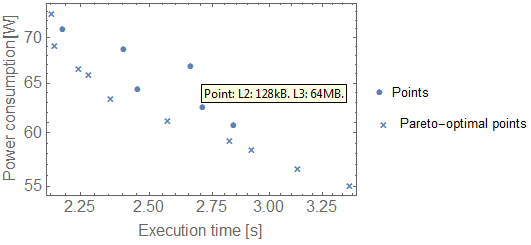
\includegraphics[width=0.8\columnwidth]{img/DSEexample.png}
 \caption{Example DSE Pareto plot.}
 \label{fig:300:dseresult}
\end{figure}

Execution of the design-space exploration can take some time as McPAT is slow to execute. Furthermore, during the design-space exploration Mathematica keeps refreshing the GUI elements in the main notebook regularly, slowing down the process. One way to somewhat speed up the design-space exploration is, after executing the main notebook (ExaBoundsLite.nb) once, to remove the output cells of that notebook. Go to ExaBoundsLite.nb, and select in the \emph{Cell} menu \emph{Delete All Output}. This removes all GUI elements (and they subsequently cannot be used anymore), but IBM ExaBounds stays live in the kernel.

\subsection{Network and full-system design-space exploration}
First we provide an example of a design-space exploration study across different network configurations. The performance metric is the communication time. We assume that the user has an extrapolated profile for an application with one single cluster of MPI processes and a \textit{uniform} communication pattern, such as Graph 500.

The user defines the network architecture properties and the mapping of MPI processes to nodes. 
\begin{mma}
	\In |ExaBoundsState = SetKeyValue[ExaBoundsState|, \linebreak \mathtt{"}|networkConfiguration|\mathtt{"}, \mathtt{"}|fat-tree-3L|\mathtt{"}]; \\
	\In	|ExaBoundsState = SetKeyValue[ExaBoundsState|, \linebreak \mathtt{"}|mappingDescription|\mathtt{"}, <\mid \mathtt{"}|type|\mathtt{"} \rightarrow \mathtt{"}|linear|\mathtt{"} \mid>]; \\
	\In	|ExaBoundsState = SetKeyValue[ExaBoundsState|, \linebreak \mathtt{"}|nodeStackLatency|\mathtt{"}, 0.0000009]; 				\\
	\In	|ExaBoundsState = SetKeyValue[ExaBoundsState|, \linebreak \mathtt{"}|switchLatency|\mathtt{"}, 0.0000007]; 					\\
	\In	|ExaBoundsState = SetKeyValue[ExaBoundsState|, \linebreak \mathtt{"}|switchSwitchBandwidth|\mathtt{"}, 5*1024*1024*1024]; 	\\
	\In	|ExaBoundsState = SetKeyValue[ExaBoundsState|, \linebreak \mathtt{"}|nodeSwitchBandwidth|\mathtt{"}, 5*1024*1024*1024];  	\\
	\In	|ExaBoundsState = SetKeyValue[ExaBoundsState|, \linebreak \mathtt{"}|nodeSwitchLinkLatency|\mathtt{"}, 0.0000000025];  		\\
	\In	|ExaBoundsState = SetKeyValue[ExaBoundsState|, \linebreak \mathtt{"}|switch1Switch2LinkLatency|\mathtt{"}, 0.000000012]; \\
\end{mma}

The user also defines the variations of network architectures to be analyzed. Let's assume that the user analyzes multiple network scenarios of fat-tree-3L topologies for an application with 262144 MPI processes. IBM ExaBounds currently supports assigning one MPI process per node (single-threaded process) and the number of nodes needs to be equal to the number of MPI processes, meaning that the system is fully populated. For a fat-tree-3L, the number of nodes is equal to m1$\cdot$m2$\cdot$m3 which, in this example, should be 262144.
\begin{mma}	
	\In |w0 = \{1, 1, 1, 1\}|; 			\\
	\In	|w1 = \{64, 16, 128, 32\}|; 	\\
	\In	|w2 = \{64, 16, 64, 32\}|; 		\\
	\In	|m1 = \{64, 64, 128, 256\}|; 	\\
	\In	|m2 = \{64, 64, 32, 32\}|; 		\\
	\In	|m3 = \{64, 64, 64, 32\}|; 		\\
	\In |ft3LConfs = Transpose[\{w0, w1, w2, m1, m2, m3\}]|; \\
\end{mma}

For each of the four network scenarios defined above, the user can retrieve the communication time as follows. 
\begin{mma}	
	\In |Do|[\linebreak
		|swProfile = SetKeyValue[swProfile, "topologyDescription"|, \linebreak <\mid \mathtt{"}w0\mathtt{"} \rightarrow |conf[[1]]|, \mathtt{"}w1\mathtt{"} \rightarrow |conf[[2]]|, \mathtt{"}w2\mathtt{"} \rightarrow |conf[[3]]|, \linebreak \mathtt{"}m1\mathtt{"} \rightarrow |conf[[4]]|, \mathtt{"}m2\mathtt{"} \rightarrow |conf[[5]]|, \mathtt{"}m3\mathtt{"} \rightarrow |conf[[6]]| \mid>]; \\
	\In |commTime = GetCommunicationTime[ExaBoundsState, swProfile]|; \\
	\quad , \{conf, ft3LConfs\} ];
\end{mma}

The example above is a simple design-space exploration across the parameters that describe the network topology (in the case of fat-tree-3L, these parameters are w0, w1, w2, m0, m1 and m2). The user can extend this study with more hardware parameters such as latencies or bandwidths.

\vspace{0.5cm}
\begin{minipage}[t]{0.05\textwidth}
	~\\
	\Huge !
\end{minipage}
\begin{minipage}[t]{0.94\textwidth}
	For the network models, IBM ExaBounds currently assumes that all links between switches have the same latency and the same bandwidth. It can be however easily extended to support multiple latencies and bandwidths. Moreover, if the user gets a \textit{missingModel} warning, the user should double-check the name of the topology and the name of the communication pattern. If the topology name or communication pattern is not recognized, IBM ExaBounds does not exit, but prints a warning (Missing model for \textit{topology}: "average link latency", "average number of links", "effective bandwidth").	Thus, the user should always check the warnings.\\
\end{minipage}

Next, to estimate the power consumption of a full system (processors and network), the user must first calculate the processor time (compute, \textit{compTime}) and the network time (communication, \textit{commTime}). In this example, there is only one class of processes, thus we calculate the compute and communication times once (per hardware architecture) and add them to estimate the execution time of the MPI application. This model is reasonable for HPC applications which are typically programmed in a way that minimizes the waiting times and the data dependencies between processes.  If there are multiple classes (clusters) of processes, the user should 1. calculate the compute and communication times per cluster, 2. add them to estimate the time of the process representative of the cluster and 3. estimate the execution time of the MPI application by calculating the maximum time across clusters. This is one possible model to predict application time performance. The user is however free to use any other model for estimating the application time, starting from the IBM ExaBounds processor and network estimates per process or cluster.

In the following we show how the user can estimate the power consumption of the full system (an application with one cluster of MPI processes).
\begin{mma}
	\In |procs = m1*m2*m3|; \\
	\In |appTime = compTime + commTime|; \\
	
	\In	|compPower = Poweri[SocketLayer[], ExaBoundsState, swProfile, False]|; \\
	\In |compPowerStatic = powerProcMem[[1]]|; \\
	\In |compDynamicPower = powerProcMem[[2]]|; \\
	\In |compStaticEnergy = procs*compPowerStatic*appTime|; \\
	\In |compDynamicEnergy = procs*compPowerDynamic*compTime|; \\
	
	\In |commDynamicEnergy = | \linebreak |procs*GetNetworkDynamicEnergy[ExaBoundsState, swProfile]|; \\
	\In |commStaticEnergy = | \linebreak |GetNetworkStaticEnergy[ExaBoundsState, swProfile, appTime]|; \\
	
	\In |systemPower = (compStaticEnergy + compDynamicEnergy +| \linebreak | commStaticEnergy + commDynamicEnergy)/appTime| \\
\end{mma}

The design-space exploration presented at the beginning of this section could be easily extended with the power analysis above so that the user can perform a complete power-performance trade-off analysis. 
